\documentclass[10pt,paper=letter]{scrartcl}
\usepackage[alttitle]{cjquines}

\begin{document}

\title{VCSMS PRIME}
\subtitle{Program for Inducing Mathematical Excellence}
\author{Session 10: Polynomials}
\date{October 13, 2017}

\maketitle
\setlength{\unitlength}{1in}
\begin{picture}(0,0)
  \put(5.5,0.5){\hbox{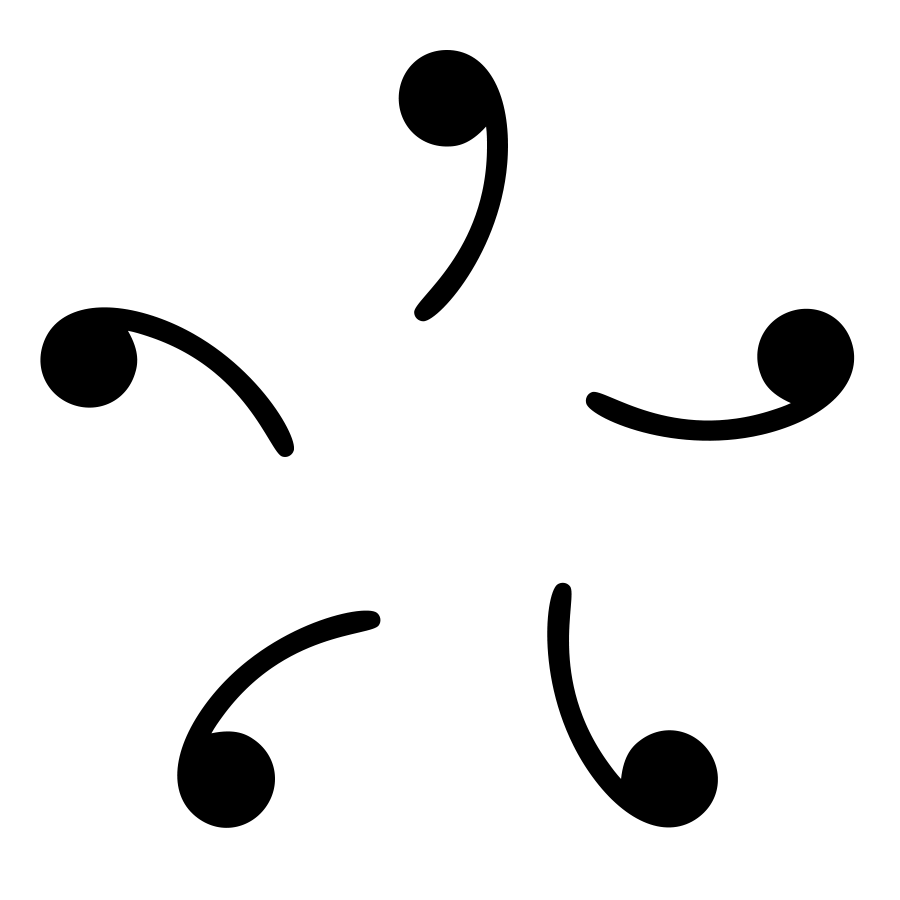
\includegraphics[width=0.9in]{logo.png}}}
\end{picture}
\vspace{-3.5em}

\subsubsection*{Lecture problems}

\begin{enumerate}
  \item What is $(1 + i)^{2017}$?
  \item A robot's first move is to go east one unit. For its $n+1$st move, it turns $45\dg$ counterclockwise and travels half the distance of the $n$th move. How far is the robot from where it started after $2017$ moves?
  \item Complex numbers $x, y, z$ satisfy $\abs{x} = \abs{y} = \abs{z} = xyz = 1$ and $x + y + z = 0$. Find $\abs{(2+x)(2+y)(2+z)}$.
  \item (MMC) A third-degree polynomial satisfies $P(0) = -3$ and $P(1) = 4$. When $P(x)$ is divided by $x^2 + x + 1$ the remainder is $2x - 1$. In the same division, what is the quotient?
  \item (USAMO) Let $a, b, c, d$ be real numbers such that $b - d \geq 5$ and the zeroes $x_1, x_2, x_3, x_4$ of the polynomial $P(x) = x^4 + ax^3 + bx^2 + cx + d$ are real. Find the minimum of $\del{x_1^2 + 1}\del{x_2^2 + 1}\del{x_3^2 + 1}\del{x_4^2 + 1}$.
  \item Prove that $\sin\del{\pi/n}\sin\del{2\pi/n}\cdots\sin\del{(n-1)\pi/n} = n/2^{n-1}$.
  \item (QII3) Let $f(x)$ be a polynomial of degree $4$ with integer coefficients, leading coefficient $1$, and having $\sqrt{10} + \sqrt{11}$ as one of its zeroes. What is the sum of its coefficients?
  \item (MMC) Find the $x$-coefficient of the fifth-degree polynomial satisfying $P(3^k) = k$ for $k = 0, 1, \ldots, 5$.
  \item (AIME II 2005/13) Let $P(x)$ be a polynomial with integer coefficients satisfying $P(17) = 10$ and $P(24) = 17$. Given $P(n) = n + 3$ has two distinct integer solutions, find their product.
  \item (QI4) Suppose that $r_1$ and $r_2$ are the roots of the equation $4x^2 - 3x - 7 = 0$. What is the sum of the squares of the reciprocals of $r_1$ and $r_2$?
  \item (Mandelbrot) Find the area of the triangle whose side lengths are the roots of $x^3 - 4x^2 + 5x - 1.9$.
  \item (AIME 2005/8) Find the sum of the roots of the equation $2^{333x-2} + 2^{111x+2} = 2^{222x+1} + 1$.
\end{enumerate}

\subsubsection*{Completing the reals}

\begin{itemize}
  \item The algebraic completion of the reals are the complex numbers. That is, any polynomial with real coefficients has only complex roots. The complex numbers are algebraically closed.
  \item We can represent as $z = a + bi$ and think of it as Cartesian coordinates, or $re^{i\theta} = r\del{\cos\theta + i \sin\theta} = r\cis\theta$ and think of it as polar coordinates. The latter is often more helpful.
  \item We write $\abs{z} = r$ and $\arg z = \theta$. Its conjugate is written as $\bar{z} = a - bi$ and has the important property $\abs{z}^2 = z\bar{z}$. Conjugation distributes over arithmetic.
  \item Addition is vectorially or end-to-end. Multiplication is rotation and scaling: the radii multiply, the directions add because of $re^{i\theta}$. This gives de Moivre's theorem.
  \item Problem 1: It would be hard to expand, so instead use polar coordinates: $\del{\sqrt2\cis45\dg}^{2017}$.
  \item Problem 2: Represent each move with complex numbers, it's the previous move times $\frac{\sqrt2}4(1+i)$. It's a geometric series with first term $1$ and $2017$ terms. Compute its sum using problem $1$.
\end{itemize}

\newpage

\subsubsection*{Roots of unity}

\begin{itemize}
  \item The $n$th roots of unity are the $n$ complex roots to $x^n - 1 = 0$. The square roots of unity are $1$ and $-1$, the cube roots are $1$, $\cis\frac{2\pi}{3}$, and $\cis\frac{4\pi}{3}$, the fourth roots are $1$, $i$, $-1$, and $-i$. Generally, $n$th roots of unity are $\cis\del{\frac{2\pi}{n}k}$ for nonnegative $k$ less than $n$.
  \item Typically: $x^3 = 1$ but $x \neq 1$. Then if you let $\omega$ be the first cube root, $\omega^2$ is the second cube root. Also $x^3 - 1 = (x - 1)(x^2 +x + 1) = 0$, but $x \neq 1$, so $\omega^2 + \omega + 1 = 0$ as it is a root.
  \item Problem 3: If you see symmetric relations involving complex numbers, guess roots of unity. Which works here, luckily: $x = 1, y = \omega, z = \omega^2$ works. Then expand.
\end{itemize}

\subsubsection*{Polynomial division}

\begin{itemize}
  \item The division algorithm is $P(x) = Q(x)D(x) + R(x)$ with obvious relations between degrees. The remainder theorem and factor theorem follow from $D(x) = x-a$ and substitution.
  \item Problem 4: Write $P(x) = Q(x)(x^2 + x + 1) + (2x - 1)$, then $Q(x)$ is linear, substitute $x = 0, 1$.
\end{itemize}

\subsubsection*{Factored form}

\begin{itemize}
  \item An $n$th degree polynomial can be written as $\prod(x-r_i)$, where $r_i$ are its roots. This goes with substitution. Interpreting factors gives the table of signs, relative maxima and minima, etc.
  \item Problem 5: Thinking $P(x) = \prod\del{x - x_i}$ and factoring $\prod\del{x_i^2 + 1} = \prod \del{x_i - i}\del{x_i + i}$, we get the inspiration to write the product as $P(i)P(-i)$. The product is at least $16$ from the inequality, and it's achievable when all the roots are $1$.
  \item Problem 6: Let $\omega = e^{i\pi/n}$. Recall from session 5 that $\sin(k\pi/n) = (\omega^k - \omega^{-k})/2i$. Then the product is $\prod_{k = 1}^{n-1}\frac{\omega^k - \omega^{-k}}{2i} = \frac1{2^{n-1}}\prod_{k=1}^{n-1} \frac{\omega^{-k}}{i}\del{1 - \omega^{2k}}.$ The left factor is just $\omega^{-n(n-1)/2}$ divided by $i^{n-1}$, which cancels. The right factor is substituting $1$ in the roots of unity polynomial $x^n - 1 = 0$, $x \neq 1$.
\end{itemize}

\subsubsection*{Root theorems}

\begin{itemize}
  \item Polynomials with real coefficients have conjugate non-real roots, polynomials with rational coefficients have conjugate irrational roots. Also, rational root theorem and synthetic division for root-finding.
  \item Problem 7: The roots are $\pm\sqrt{10}\pm\sqrt{11}$. Its sum of coefficients is $f(1)$, think of its factored form. Or, do $x = \sqrt{10} + \sqrt{11}$ and square twice.
\end{itemize}

\subsubsection*{Rewriting polynomials}

\begin{itemize}
  \item Problem 8: Consider the polynomial $P(3x) - P(x) - 1$. It is a fifth-degree polynomial with roots $k = 1, \ldots, 5$, so we can write it as $A(x-1)(x-2)\cdots(x-5)$ for some constant $A$. Substituting $x=0$ gives the constant, and we only need to find the $x$-coefficient.
  \item Problem 9: We have $P(x) - x + 7 = A(x)(x-17)(x-24)$, also $P(x) - x - 3 = B(x)(x-n_1)(x-n_2)$. Then $n_1$ and $n_2$ are the roots of $A(x)(x-17)(x-24) = 10$, trial and error gives $n = 19, 22$.
\end{itemize}

\subsubsection*{Roots and coefficients}

\begin{itemize}
  \item Vieta's, rule of signs, discrete Fourier: ``find the sum of the coefficients with exponent divisible by 3.''
  \item Problem 10: Directly, $1/r_1^2 + 1/r_2^2 = (r_1 + r_2/r_1r_2)^2 - 2/(r_1r_2)$. There is also an important trick: for a bijection $f$, the substitution $x \to f^{-1}(x)$ changes the roots to $f(r_i)$. So here, we can try $x \to 1/x$. 
  \item Problem 11: Recall Heron's and factored form. The semiperimeter is half the sum of the roots, or $2$. 
  \item Problem 12: Substitute $2^{111x} \to y$. The sum of $x$ is the sum of $\frac1{111} \log_2 y$, so Vieta's on products.
\end{itemize}

\end{document}
